\documentclass[tikz,border=4pt]{standalone}
\usepackage[T1]{fontenc}
\usepackage{amsmath}
\usetikzlibrary{positioning,arrows.meta,calc,fit,backgrounds}
\definecolor{ink}{HTML}{0B0B0B}
\definecolor{ink2}{HTML}{52514E}
\definecolor{adj}{HTML}{2A78D6}
\definecolor{adjl}{HTML}{CDE2FB}
\definecolor{pinn}{HTML}{EB6834}
\definecolor{pinnl}{HTML}{FBDCCC}
\definecolor{neut}{HTML}{F1F0EC}
\begin{document}
\sffamily
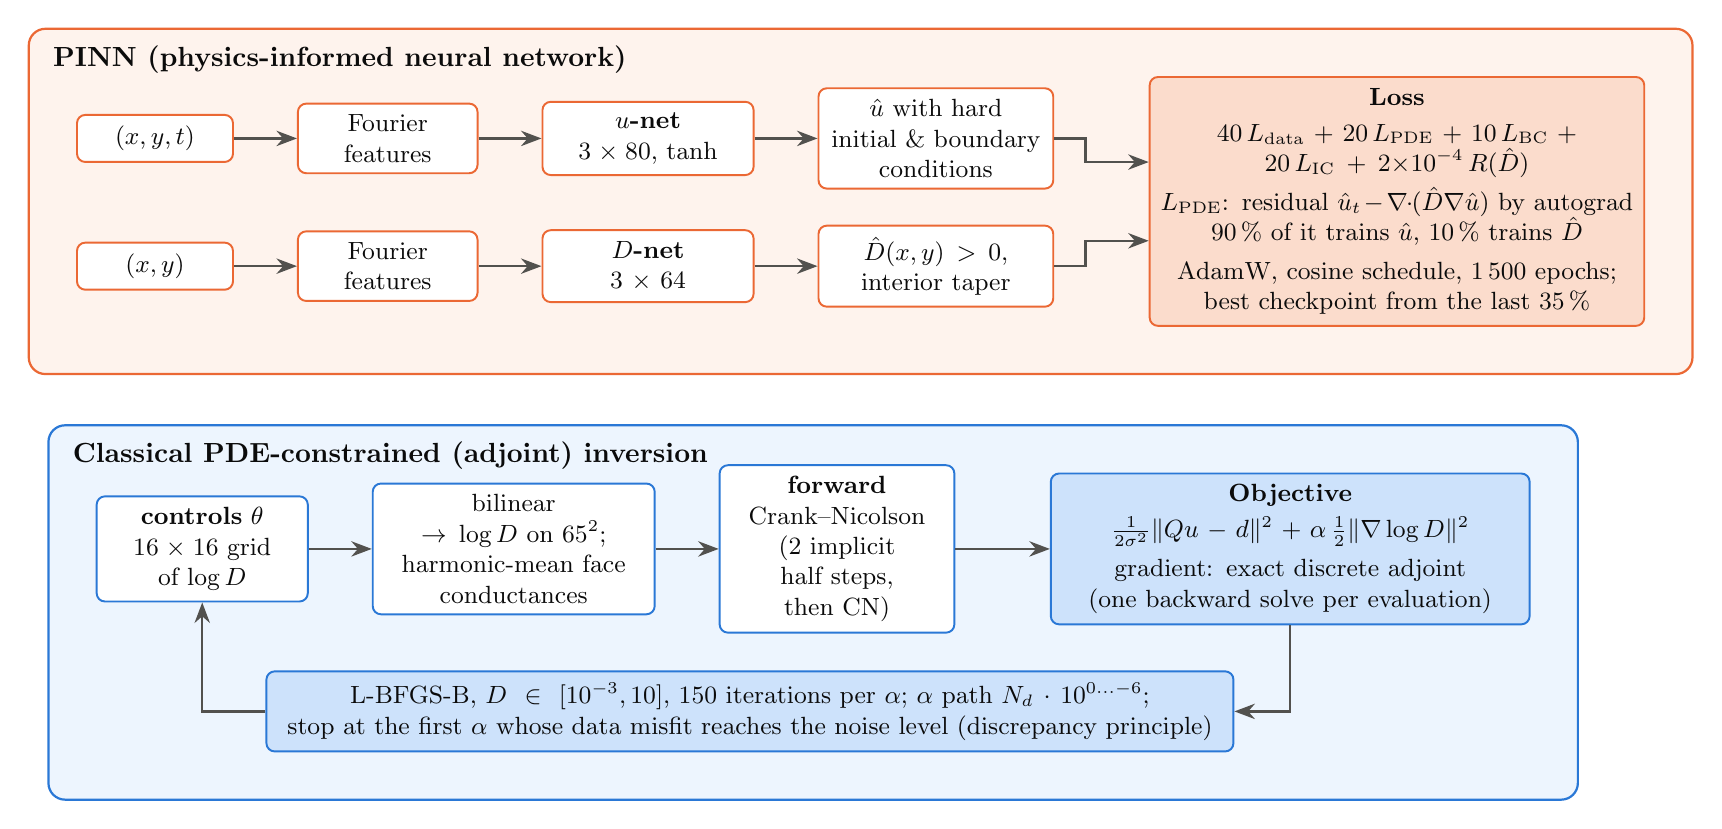
\begin{tikzpicture}[
  node distance=6mm and 8mm,
  b/.style={draw=#1, line width=0.7pt, rounded corners=3pt, fill=white, align=center, inner sep=4pt,
            font=\small\color{ink}},
  b/.default=ink2,
  arr/.style={-{Stealth[length=2.6mm]}, line width=0.9pt, draw=ink2},
  ttl/.style={font=\normalsize\bfseries\color{ink}, anchor=west}]

% ------------------------------------------------------------------ PINN
\node[b=pinn, text width=17mm] (xyt) {$(x, y, t)$};
\node[b=pinn, text width=20mm, right=of xyt] (ffu) {Fourier\\features};
\node[b=pinn, text width=24mm, right=of ffu] (unet) {{\bfseries $u$-net}\\$3\times80$, tanh};
\node[b=pinn, text width=27mm, right=of unet] (uhat) {$\hat u$ with hard\\initial \& boundary\\conditions};

\node[b=pinn, text width=17mm, below=10mm of xyt] (xy) {$(x, y)$};
\node[b=pinn, text width=20mm, right=of xy] (ffd) {Fourier\\features};
\node[b=pinn, text width=24mm, right=of ffd] (dnet) {{\bfseries $D$-net}\\$3\times64$};
\node[b=pinn, text width=27mm, right=of dnet] (dhat) {$\hat D(x,y)>0$,\\interior taper};

\draw[arr] (xyt) -- (ffu); \draw[arr] (ffu) -- (unet); \draw[arr] (unet) -- (uhat);
\draw[arr] (xy) -- (ffd); \draw[arr] (ffd) -- (dnet); \draw[arr] (dnet) -- (dhat);

\node[b=pinn, fill=pinnl, text width=60mm, right=12mm of uhat, yshift=-8mm] (loss) {
  {\bfseries Loss}\\[2pt]
  $40\,L_{\mathrm{data}} + 20\,L_{\mathrm{PDE}} + 10\,L_{\mathrm{BC}} + 20\,L_{\mathrm{IC}} + 2{\times}10^{-4}\,R(\hat D)$\\[3pt]
  $L_{\mathrm{PDE}}$: residual $\hat u_t - \nabla\!\cdot\!(\hat D\nabla\hat u)$ by autograd\\
  90\,\% of it trains $\hat u$, 10\,\% trains $\hat D$\\[3pt]
  AdamW, cosine schedule, 1\,500 epochs;\\best checkpoint from the last 35\,\%};
\draw[arr] (uhat.east) -- ++(4mm,0) |- ([yshift=5mm]loss.west);
\draw[arr] (dhat.east) -- ++(4mm,0) |- ([yshift=-5mm]loss.west);

\begin{scope}[on background layer]
  \node[fit=(xyt)(dhat)(loss), inner sep=6mm, fill=pinnl!35, rounded corners=6pt, draw=pinn, line width=0.8pt] (pbox) {};
\end{scope}
\node[ttl, text=pinn!80!black] at ([xshift=2mm, yshift=-1mm]pbox.north west) [anchor=north west] {\color{ink}PINN (physics-informed neural network)};

% ------------------------------------------------------------------ adjoint
\node[b=adj, text width=24mm, below=26mm of xy, xshift=6mm] (theta) {{\bfseries controls $\theta$}\\$16\times16$ grid\\of $\log D$};
\node[b=adj, text width=33mm, right=of theta] (fv) {bilinear $\to \log D$ on $65^2$;\\harmonic-mean face\\conductances};
\node[b=adj, text width=27mm, right=of fv] (cn) {{\bfseries forward}\\Crank--Nicolson\\(2 implicit half steps,\\then CN)};
\node[b=adj, fill=adjl, text width=58mm, right=12mm of cn] (obj) {
  {\bfseries Objective}\\[2pt]
  $\tfrac{1}{2\sigma^2}\lVert Q u - d\rVert^2 + \alpha\,\tfrac12\lVert\nabla\log D\rVert^2$\\[3pt]
  gradient: exact discrete adjoint\\(one backward solve per evaluation)};

\node[b=adj, fill=adjl, text width=120mm, below=7mm of fv, xshift=30mm] (opt) {
  L-BFGS-B, $D\in[10^{-3}, 10]$, 150 iterations per $\alpha$; $\alpha$ path $N_d\cdot10^{0\ldots-6}$;\\
  stop at the first $\alpha$ whose data misfit reaches the noise level (discrepancy principle)};

\draw[arr] (theta) -- (fv); \draw[arr] (fv) -- (cn); \draw[arr] (cn) -- (obj);
\draw[arr] (obj.south) |- (opt.east);
\draw[arr] (opt.west) -| (theta.south);

\begin{scope}[on background layer]
  \node[fit=(theta)(obj)(opt), inner sep=6mm, fill=adjl!35, rounded corners=6pt, draw=adj, line width=0.8pt] (abox) {};
\end{scope}
\node[ttl] at ([xshift=2mm, yshift=-1mm]abox.north west) [anchor=north west] {Classical PDE-constrained (adjoint) inversion};
\end{tikzpicture}
\end{document}
